% {{{=================== Introduction ======================


\section{Introduction}

\subsection{Motivation}
\UH{}\footnote{Unknown Horizons website: \url{http://www.unknown-horizons.org}} is an \OS{} real-time strategy game developed by a team of programmers, artists, game
designers and many more around the globe. The first revision to the current project was committed in late 2007\footnote{First commit to \UH{}:
\url{https://github.com/unknown-horizons/unknown-horizons/commit/53eec12fd8bb52ac1a6ccfdb097296c479499dfd}}. The idea
started out in 2005 under the name \textit{OpenAnno} and was renamed to \UH{} in early 2009.

Over the years the project grew to a small team of more than 10 active developers and many
patch contributors. The recent release version of \UH{} has been downloaded more than 10000 times\footnote{Sourceforge
download statistics:
\url{http://sourceforge.net/projects/unknownhorizons/files/Unknown\%20Horizons/2011.2/}}\footnote{Chip.de download
statistics: \url{http://www.chip.de/downloads/Unknown-Horizons_33713541.html\#sp=unknown horizons\&N=0\&pos=1}}, a rather
big user-base compared to the team size.

In this document I want to give a personal report on the work I have done on \UH{} in the past years and give an
overview of how certain parts of the project's organization have evolved.

\subsection{About Me}
My name is Thomas Kinnen, I'm currently doing my Masters in Computer Science. On the development team and in the code
repository I am mostly known by the nick-name \textit{nihathrael}.

I started working on the project in early 2008, shortly after the first commits had been commited to the repository. 
The project had nearly come to a complete halt when I joined, so I set out to bring it back to life.

Since November 2008 I am one of the two project coordinators, with focus on code direction and introduction of new
potential members to the team and code. In this position I got a good view into most of the necessary parts of an \OS{}
game development team. This includes public relations, mentoring new members, graphics, content, programming, code
design, leading meetings and many more.

\section{History}
In this section I present the history before and during my time as part of the \UH{} team. I give only a brief
overview of the history before I joined the project, as the current state has nothing, but the idea, in common with the
older versions.

\subsection{Pre History}
The idea for the \UH{} project existed long before I joined the team in 2008. The project's first name was \textit{OpenAnno}
for which the original sourceforge.net project was registered as early as July 2005\footnote{Original sourceforge.net
project: \url{http://sourceforge.net/projects/openanno/}}. The original announcement for OpenAnno can be found on the
German Linux forums: \url{http://linuxforen.de/forums/showthread.php?t=188350}. Version 3.5 (See screenshot in \figref{oascreenshot}) of OpenAnno was released in
early 2006\footnote{Link to a download site: \url{http://happypenguin.org/newsitem?id=6154}}. After a rewrite to C++,
version 0.0.1.0 of OpenAnno was released in September 2006\footnote{Release announcement 0.0.1.0:
\url{http://da.zfx.info/developia/viewarticlecomments.php?cid=28999\#29101}}. 

\begin{figure}[!htb]
	\begin{center}
		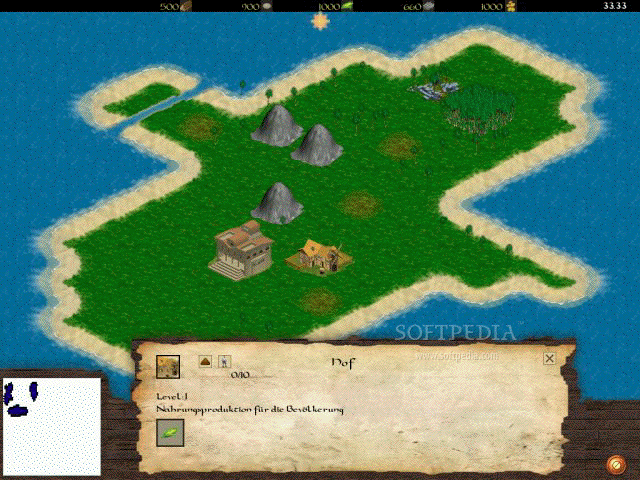
\includegraphics[scale=0.50]{pics/openannoscreenshot}
	\end{center}
    \caption{Early screenshot from OpenAnno 3.5 - taken from
    \href{http://mac.softpedia.com/progScreenshots/OpenAnno-Screenshot-13550.html}{Softpedia.com}}
    \label{oascreenshot}
\end{figure}

In April 2007 \textit{LinuxDonald}(Thomas Kowaliczek) took over the project from
\textit{The Brain}(Martin Gerhardy)\footnote{Original Blog post by LinuxDonald (German):
\url{http://www.linuxdonald.de/blog/?p=4}}.

The project took an interesting turn in August 2007 when the team decided to
split the project into a 2D and a 3D version\footnote{Splitting 2D/3D blog post:
\url{http://www.linuxdonald.de/blog/?p=13}}.

OpenAnno 2D was restarted in September 2007, using FIFE\footnote{FIFE
website \url{httpd//www.fifengine.net}} as its graphics engine. The team was hoping the collaboration with a dedicated
graphics engine would make their work easier, as they had previously stalled on implementing different terrain heights
and where having trouble getting all the work done. OpenAnno 3D was dropped in the same decision as the team had
realized that the burden of developing two games basically in parallel was not a viable option. This presented a radical
cut in the development of OpenAnno, as the core repository had over 1000 commits at that time\footnote{Blog post about
the 1000th commit: \url{http://www.linuxdonald.de/blog/?p=6}}. Restarting meant throwing years of development over board
to start again from scratch.

\subsection{History - 2008}
In March 2008 I joined the project as a novice programmer. When I joined the project, it had almost come to a halt. Amazed
by the idea of writing an \OS{} game in the footsteps of \textit{Anno 1602} I decided to give it a try non-the-less. The
entire code was removed and I started from scratch, using only the graphics from old versions. Motivated by the new start
\textit{spq}(Kristoffer Janke) quickly joined me in my efforts only 18 days later. \textit{spq} and I had a lot of time at our disposal, so with
the help of many other old and new members development of \textit{OpenAnno} progressed quickly. We hit 500 commits to the repository
by June 2008 and finished our first milestone \textit{2008.0} by July 8th. The 1000. commit followed quickly by July 16th. At the
end of July the team had its first meet-up at the \textit{Dusmania 2008} hobby game developers conference and was awarded
2nd place in the category best game.

On October 1st \textit{OpenAnno} hit a major milestone with its first public release: \textit{Version 2008.1}. The release
received quite a lot of coverage and was featured on some big websites like the German magazine chip.de\footnote{Chip news entry to
2008.1:\url{http://www.chip.de/news/OpenAnno-Strategiespiel-Klassiker-als-Open-Source_33713075.html\#sp=openanno&N=0&pos=1}}
and the freegamer blog\footnote{Freegamer blogpost: \url{http://freegamer.blogspot.com/2008/10/lavirinto-3d-060-balazar-3-01-openanno.html}}

During this time it became clear that \textit{LinuxDonald} would not be able to continue doing the project management
due to a lack of time on his side. After a long meeting and a vote at the beginning of November it was decided to split the
position in two team coordinator jobs. \textit{Nightraven} (Tobias Schröfel) was assigned to public relations and
advertising and guiding game design decisions. I was chosen to assign tasks and guide the development of the code base.
Tasks for both project coordinators were defined as posting news updates, guiding discussion on IRC and helping new
interested developers join our project. LinuxDonald agreed to continue hosting the website and repository
infrastructure, showing it was not the lack of interest but the lack time that caused him to step down.

\subsection{History - 2009}
The year 2009 started with a big change: The project was renamed to \UH{}. This was done for two reasons:
\begin{itemize}
    \item Copyright concerns about the word "Anno" being licensed by \textit{Sunflowers} in Germany
    \item Separate the game from the original Anno series, underlining it not being a clone
\end{itemize}

As \UH{} is not a formal organization or company any lawsuits against the name (or any other port of the project) would
result in the lawsuit going against the project coordinators Nightraven and/or me. Therefor we decided to change the name to
something completely new, leaving us on the safe side of things.

This is the original commit from the official repository performing the renaming:
\begin{lstlisting}[caption=Commit 1831 renaming OpenAnno to Unknown Horizons, label=renamecommit]
Author: nihathrael
Date:   Fri Feb 20 16:39:37 2009 +0000
    * Renamed all occurrences of OpenAnno to Unknown Horizons
    * openanno.py is now named run_uh.py
    * openanno.sqlite ist now named game.sqlite
    * Goodbye OpenAnno ;( Off to new shores we go :)
\end{lstlisting}

Besides this big change, 2009 was a regular development year for \UH{}. The team released three new versions of \UH{}:
\begin{itemize}
\item \textit{2009.0}
\item \textit{2009.1}
\item \textit{2009.2} + bugfix release \textit{2009.2a}. 
\end{itemize}
The releases generated over 35 thousand downloads on sourceforge alone.

The release 2009.2 was featured in the big German computer magazine \textit{c't}\footnote{\url{http://www.heise.de/software/download/cdd_95_9}} and was delivered with the magazine's
DVD, which is shipped with each copy. 

\pagebreak

\subsection{History - 2010}
In 2010 the team decided to move away from the subversion\footnote{\url{http://subversion.tigris.org}} revision control
system and switch to git\footnote{\url{http://git-scm.com/}}. With this switch, the repository hosting was also moved to
\href{http://www.github.com}{github.com}. Github is a collaborative source-code hosting website which deeply integrates
git into the website. It makes it easy for developers to submit patches and even easier for the team to merge it. This
also moves the source-code hosting away from our own servers, making it much more reliable and cheaper.

The team shipped one release: Version \textit{2010.1}. It introduced a network mode, allowing the player
to play with other players over the internet or a local area network.

\subsection{History - 2011}
2011 has been an exciting year for \UH{} so far. Early 2011 the team decided to apply for the \textit{Google Summer of
Code}\footnote{Official GSoC website: \url{http://www.google-melange.com/gsoc/homepage/google/gsoc2011}} program. The
application was accepted and \UH{} was granted 3 student slots. The team had applied together with the graphics engine
\textit{FIFE} and it was decided that 1 slot would go to \textit{FIFE} and 2 to \UH{}. The three students were chosen
for the following projects:
\begin{itemize}
    \item Artificial Intelligence Player for \UH{}
    \item Combat for \UH{}
    \item Performance Improvements for the Rendering Pipeline in \textit{FIFE}
\end{itemize}
Before the students started their work, the team released versions \textit{2011.1} and \textit{2011.2} of \UH{}.

The students did excellent work during the three months of their active work on both \UH{} and \textit{FIFE} and all
easily passed the final evaluation. Following up on the \textit{Summer of Code} Google invited two members of each
organization to participate in the mentor summit at their campus in Mountain View. Christoph Ölmüller, who did the
administrative work for GSoC for \UH{}, and me got the chance to go and meet many fellow \OS{} game developers
from other projects like \BOW{}, \textit{Worldforge} and \textit{Hedgewars}.

\begin{figure}[!htb]
	\begin{center}
		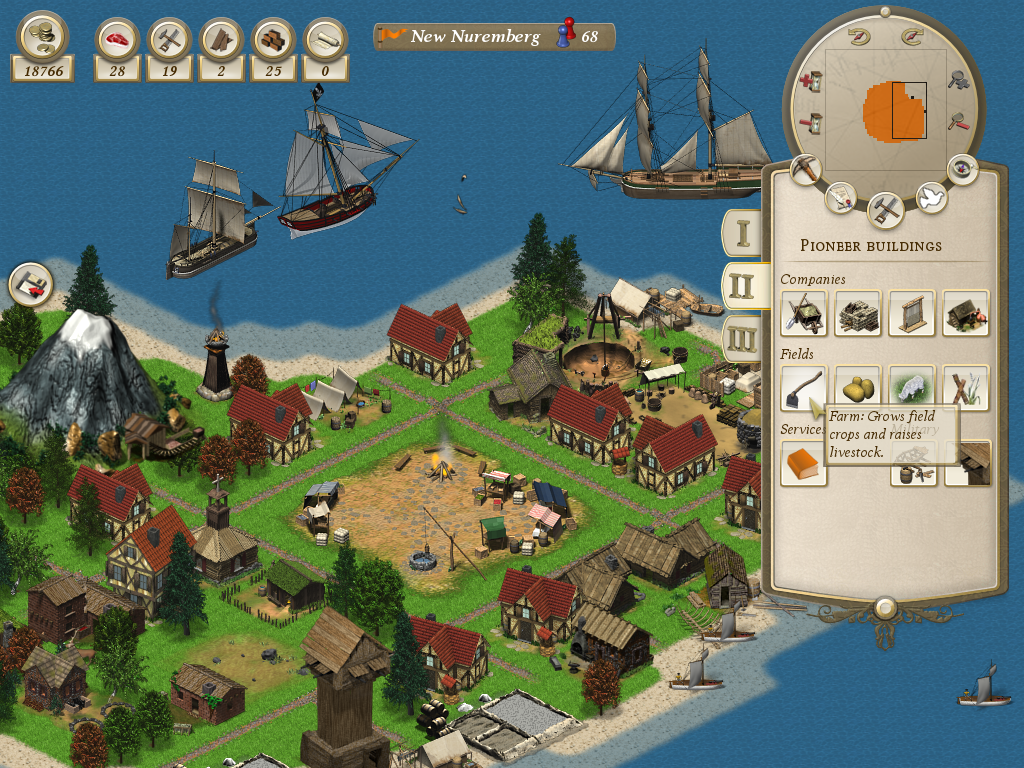
\includegraphics[scale=0.28]{pics/uhscreenshot}
	\end{center}
    \caption{Screenshot of the upcoming \UH{} release version 2011.3}
    \label{uhscreenshot}
\end{figure}

\textit{FIFE} released version \textit{0.3.3} of their engine on October 7th,
followed by bugfix release \textit{0.3.3r2} on November 2nd. This release includes all changes done by their student
\textit{kozmo} (Kajetan Świerk). \UH{} will release \UH{} version 2011.3 during the 2nd week of November, containing all
changes made during the \textit{Summer of Code} and the regular development (See \figref{uhscreenshot}).


\section{Project Organization}
In this section a description on how the project's members are structured and how the project is organized using
different tools like meetings and bug trackers.

\subsection{Member structure}
There are only two defined jobs on the team: The two project coordinator jobs held by \textit{Nightraven} and me. It was
specifically named project \textit{coordinator} and not project \textit{leader} as the purpose of this position is not to
make all the decisions and tell everyone what to do. The intention is that the project coordinators guide the project on
its path, making sure basic communications work correctly. For example the project coordinators usually hold the weekly
IRC meetings and make sure the general tone of communication is friendly and helpful. This is based on the foundation
that it is not possible to force anybody to do anything on an \OS{} project, as everyone works on it in their free time
and because they enjoy it. It is the project coordinators task to make sure stays an enjoyable project to work on.

\UH{} does not follow any other strict structure of members. The team is not divided into different sub teams. Much
thought has been given the idea of forming different apartments for programming, game design and graphics but the team
found that the team size of about 10 active members is not big enough to split it into different subgroups and thereby
adding a lot of overhead to the project communications. It has been agreed that this step could be undertaken when the
project grows further and communication becomes slow if everyone talks to everyone else all the time.

Over time basic structures naturally emerged, meaning that those members spending the most time on a certain area became a
\textit{go-to} person in case of questions. For example \textit{totycro} (Bernhald Mallinger) and me are most
experienced with the code, making us the \textit{go-to} persons for this area. Since this emerged over time and is not
an artificially created structure, it automatically changes over time if new members come in and become more experienced
or are available a larger amount of the time.

\subsection{Language}
\UH{} started out as an entirely German project and remained so until I joined in 2008. It quickly became clear that a
mainly German development would not attract foreign developers easy, if at all. At the time there was only one non German
member on the team, \textit{Greyghost} (Tushar Sawant) from India, who had recently joined. He used \textit{Google
Translate} to understand wiki pages and the discussions on IRC.

The team quickly realized this would not be beneficial and decided to set English as the main language on IRC, the
website and the wiki. The change was not easy as there was some disagreement on if this was really necessary. This was one
of the main points on my personal agenda when I was voted project coordinator and is the only time I ever used my
informal ''power'' -- to enforce English language if necessary.

Today this is no longer an ongoing issue, as we have many people from countries around the world on our IRC channel,
automatically making English the language of choice.

\textit{In my opinion the decision to switch to English is the most \textbf{important and valuable} decision the team
has ever made.} It allowed us to grow the team globally and is the foundation for our participation in Google's \textit{Summer
of Code} program.

\subsection{Communication}
The team uses a variety of channels for their communication: IRC, forums, mailing-list, e-mail, etc. 
The by far most used of
these is our IRC channel \textit{\#unknown-horizons} on irc.freenode.org. As most of the developers are in a similar
timezone, real-time communication via a chat room has proven to be the best written communication available. All team members are
usually available on the IRC channel while they work on \UH{} and the team lives the habit of always being online on
IRC while in front of a computer. This way questions can usually be answered quickly and discussion is held continuously
all day around. The IRC channel is also our main support gateway for users having problems.

During the \textit{Summer of Code} we required our students join our IRC channel during their working hours, this proved
to be a very effective method of including everyone in the team and making sure the students where not a separated,
isolated group next to the team. Quickly they were actively participating in discussions and taking part in the day to
day project development.

Besides the IRC channel we also give support and collect feedback via a forum on our website\footnote{\UH{} Forum:
\url{http://forum.unknown-horizons.org/}}. Forums are the main support method in the gaming industry, which is why most
users are already accustomed to the use of a forum and find it easy to request support through this channel.

After learning about \textit{The cathedral and the bazaar}\cite{springerlink:10.1007/s12130-999-1026-0} we recently
introduced a beta mailing-list, which we recommend to users which are seeking support and are willing to put some time into
solving the problem. We post pre-releases of upcoming releases on this list, so they can be tested by a wider number
of users on different systems. This provides invaluable feedback which \textbf{can not} be replaced by any testing on our side.

We also have two more lists set up, but these are not used actively. Communication never moved from IRC to the
mailing-lists. This might very well be due to the project's size and might change if the project grows further.

\subsubsection{Weekly Meetings}
The team holds weekly meetings on IRC. These are used to discuss and decide on issues that came up during the week. It is
used to plan the upcoming tasks and distribute the workload between the members. At the end of each meeting there is a
fixed topic called \textit{Status update and Hallway chat} where everyone can drop short notes on which parts of the
project he worked this week or any other information that might be useful for the rest of the team, but does not need
discussion. This is useful to keep everyone up-to-date on how the project is going and who is doing which work.

\subsection{Tools}
The team uses many different tools to organize the development: Trac, Github and a wiki.

Trac\footnote{Trac website: \url{http://trac.edgewall.org/}} is a project management tool which allows milestone specific issue-tracking. We use it to keep track of the
different tasks and bugs that have been created and found. We also organize our planned workload for the upcoming
milestone using trac. It has proven an invaluable tool to organize the team's work.

Together with our switch to the GIT versioning system, we also switched to \href{http://www.github.com}{github.com} for the hosting. Github comes with a
number of useful tools, like providing comments on single lines in commits, which is a great tool for code review. We made
extensive use of this during our participation in \textit{Summer of Code} to give our students regular feedback on
their work.

Interested contributors can leave git pull-requests which can usually be merged by a click of a button on
the website if wanted. This has streamlined the work-flow to contribute code to our project a lot. An example for such a
pull-request can be found at: \url{https://github.com/unknown-horizons/unknown-horizons/pull/22}.

The team uses a MediaWiki\footnote{MediaWiki website: \url{http://www.mediawiki.org}} installation for documentation.
The wiki contains mostly design documentation and all sorts of
guides to help with the installation and development of the game. It is also used to store new ideas discussed on IRC
and then formulate them into something that can be implemented later on.

One thing the team learned is that trying to
maintain multiple languages of the same article in the wiki does not work with such a small team. So unless the team is
big (>100 active contributors) \textit{and} there is a very good reason to use multiple languages, I would advise the use of only
one single language (English) in the wiki.

\section{Lessons Learned}
In this section I present a few of the lessons I and/or the team have learned over the past years.

\subsection{Google Summer of Code}
Google \textit{Summer of Code} (short \textit{GSoC}) is a great opportunity for every \OS{} project to move the project
forward, gain new contributors and keep everyone motivated. It is also \textbf{a lot of work}. The application period is
already very time consuming and the mentoring part is even more so. Your project should be able to dedicate one member
for the \textit{GSoC} administration alone, he will not be doing anything else during the application process. Especially
if it is your first year participating in the project, like it was the case with \UH{} this year.

The student selection process is very difficult in my experience. Here is what we did get an idea of the applying student's
abilities:
\begin{itemize}
    \item Ask every applicant to show up on IRC. If they did not, we dismissed their proposal
    \item If they show up, ask them to fix one bug of their choice from our bug-tracker
    \item Have a nice application form to fill out\footnote{\UH{} GSoC student application form:
        \url{http://wiki.unknown-horizons.org/w/Student_application_template}}
    \item Have them summarize their proposal on our wiki
    \item Talk to each student individually about their goals, our expectations and their ideas
\end{itemize}

Of 32 applications we received in total, this process left us with 6 to decide from. The final decision is very difficult
and we let the mentor of each task decide which student he wanted to take. This is important as the mentor and the
student have to be able to
communicate well. If you have to choose between two students of which one is technically superior to the other, but
lacks communication skills, choose the one with better communication skills.

\subsection{University Projects}
There is great potential in university projects. For many subjects there are courses which demand work on a real
project. If communicated and prepared well, \OS{} projects can be these real projects. University projects generally
require quite some time on the students side, so if he can spend this time working on your project, it will gain a lot.

Our multiplayer mode is a result of such a university project -- we had totycro and two colleague working on \UH{}, for an
estimated 70 hours each. In \OS{} that is a lot of time, which is not easy to find in normal free-time.

\subsection{Keep going!}
Over the years we have had times where we hardly had one commit a week, or even a month. Do never give up! After these
times we always had times of great activity and it was well worth the effort of keeping the project running. Time is a
valuable resource on an \OS{} project and it is always scarce. People come and go, but if the project manages to keep
the core team together and motivated, work will always progress. Keep going!

\section{Conclusion}
The idea for \UH{} originated 6 years ago in the \textit{OpenAnno} project and it took 3 complete restarts to get to its
current state. Developing
a full scale RTS game is usually funded by thousand if not millions of euros, achieving the same results with an \OS{}
project is nearly impossible. Yet the team managed to build a playable game and over time became an important part of
the \OS{} gaming community. Over three years of development time have been put into the current version of \UH{} and the
project is still going forward. A low management and communication overhead is the key to keeping the project running
even in times when members are short on time.

Working on an \OS{} game has been a great experience over the past years and I am looking forward to the next years.


%}}}

